\section{Results}
\begin{table*}[t]\centering\small
\caption{Count forecasts on original final periods and fresh BPI 2012 confirmation. Lower CRPS and loss are better; nominal coverage is .90. The three factor rows retain the original individual CDFs. Revised controls on Borg/BPI 2017 are retrospective. DM development-fit scores are exact; sampled methods use 512 draws and three seeds. A dash denotes an unimplemented comparison.}\label{tab:counts}
\begin{tabular}{lrrr rrr rrr}\toprule
&\multicolumn{3}{c}{Borg}&\multicolumn{3}{c}{BPI 2017}&\multicolumn{3}{c}{BPI 2012 (fresh)}\\
Method&CRPS&Cov.&Loss$_9$&CRPS&Cov.&Loss$_9$&CRPS&Cov.&Loss$_9$\\\midrule
Independent&0.0342&0.6594&0.1311&0.0501&0.5356&0.1177&0.0716&0.4745&0.1386\\
Global factor&0.0265&0.9797&0.0551&0.0460&0.8897&0.1290&0.0625&0.8562&0.1669\\
Typed factors&0.0259&0.9059&0.0528&0.0465&0.7935&0.1222&0.0653&0.6655&0.1554\\
DM, earlier fit&0.0287&0.9342&0.0744&0.0450&0.9002&0.1287&0.0389&0.9145&0.1125\\
DM, development fit&0.0285&0.9440&0.0693&0.0408&0.9298&0.1140&---&---&---\\
Bottom-up DM&---&---&---&0.0424&0.7749&0.1326&0.0389&0.8289&0.1176\\
Conditioned DM&---&---&---&0.0418&0.7617&0.1319&0.0390&0.8125&0.1198\\
Historical residuals&0.0309&0.8746&0.0840&0.0439&0.8311&0.1258&---&---&---\\
\bottomrule\end{tabular}\end{table*}

\begin{table*}[t]\centering\small
\caption{BPI 2017 controlled same-version correction. Original Gaussian weights are fixed. These are retrospective diagnostics; improved mean calibration does not guarantee a better reserve quantile.}\label{tab:calibration}
\begin{tabular}{llrr rr}\toprule
& &\multicolumn{2}{c}{October development}&\multicolumn{2}{c}{November--December}\\
Correction&Dependence&CRPS&Loss$_9$&CRPS&Loss$_9$\\\midrule
Identity&Independent&0.0433&0.0954&0.0501&0.1176\\
Identity&Global factor&0.0410&0.1195&0.0459&0.1290\\
Identity&Typed factors&0.0411&0.1088&0.0465&0.1222\\
Static&Independent&0.0401&0.0945&0.0469&0.1197\\
Static&Global factor&0.0386&0.1147&0.0435&0.1244\\
Static&Typed factors&0.0383&0.1039&0.0439&0.1188\\
Rolling 60D&Independent&0.0401&0.0947&0.0435&0.1441\\
Rolling 60D&Global factor&0.0385&0.1146&0.0407&0.1182\\
Rolling 60D&Typed factors&0.0382&0.1037&0.0408&0.1199\\
\bottomrule\end{tabular}\end{table*}

\begin{table*}[t]\centering\small
\caption{Joint group-profile scores. ES is RMS-normalized energy score; Peak is CRPS of the maximum standardized slow-progress deviation. Scales differ across datasets. Original-period rows are retrospective; all fresh endpoints were frozen before opening February.}\label{tab:joint}
\begin{tabular}{lrr rr rr}\toprule
&\multicolumn{2}{c}{Borg}&\multicolumn{2}{c}{BPI 2017}&\multicolumn{2}{c}{BPI 2012 (fresh)}\\
Method&ES&Peak&ES&Peak&ES&Peak\\\midrule
Independent&0.0597&15.7604&0.0957&0.4613&0.1058&0.5183\\
Global factor&0.0575&7.5434&0.0942&0.4608&0.1023&0.4790\\
Typed factors&0.0546&4.1726&0.0942&0.6686&0.1015&0.7362\\
DM, earlier fit&0.0543&3.9903&0.0923&0.9984&0.0859&0.3903\\
DM, development fit&0.0544&4.0844&0.0879&0.5343&---&---\\
Bottom-up DM&---&---&0.0879&0.5380&0.0861&0.3907\\
Conditioned DM&---&---&0.0879&0.5539&0.0860&0.3922\\
Rolling correction + global&---&---&0.0880&0.4363&0.0928&0.4882\\
\bottomrule\end{tabular}\end{table*}

\begin{figure*}[t]
\centering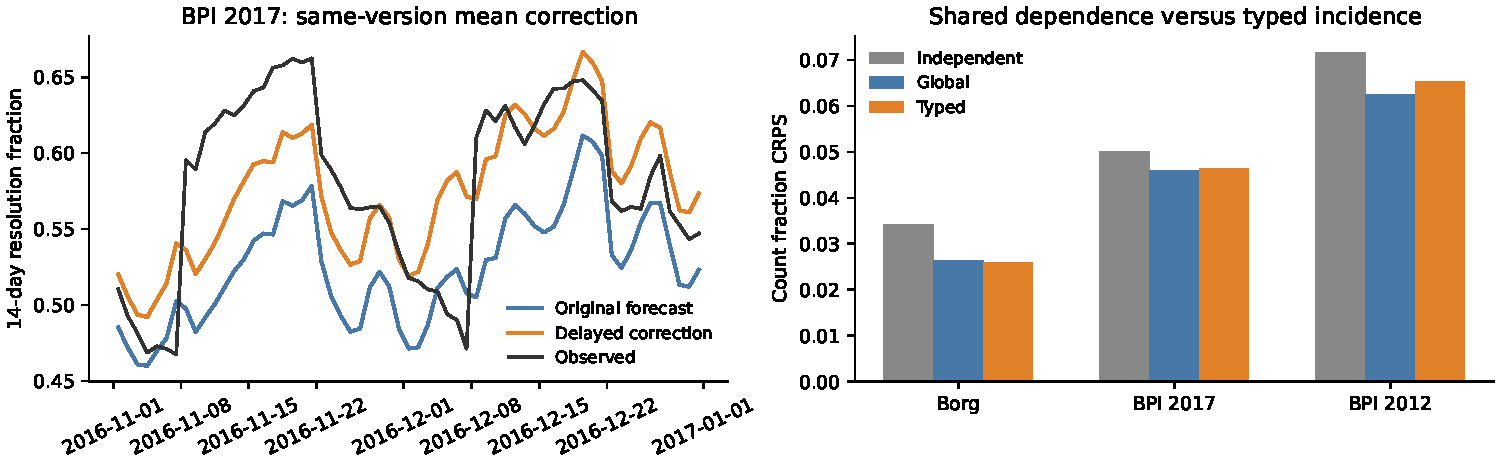
\includegraphics[width=.98\textwidth]{figures/calibration_and_controls.pdf}
\caption{Left: retrospective BPI 2017 fourteen-day population mean predictions
under original and delayed same-version correction. Right: matched-marginal
factor comparisons on original final periods and fresh BPI 2012. The global
factor captures much of the improvement over independence; typed incidence
has an application-specific incremental contribution.}
\label{fig:controls}
\end{figure*}

\subsection{Count gains survive strong controls only in some settings}
The original frozen Borg typed Gaussian model reduces count-fraction CRPS
from .03417 under independence to .02587, a 24.3\% improvement
(Table~\ref{tab:counts}). Ratio-9 reserve loss falls from .13106 to .05280.
The global factor already reaches .02646 CRPS: the additional typed gain is
2.2\%, not 24.3\%. The paired typed-minus-global CRPS interval is
$[-.00105,-.00018]$ with one-day blocks. Removing job variance increases
job-level CRPS from .01451 to .01922; removing machine variance changes
machine CRPS from .02507 to .02525. The strongest demonstrated typed signal
is therefore job grouping, with a much smaller machine contribution.

Stronger direct controls do not remove Borg's count result. The
development-fitted DM model reaches .02853 CRPS and .06931 reserve loss.
Typed-minus-DM CRPS is $-.00266$, with one-day block interval
$[-.00366,-.00169]$. The earlier-OOF DM and historical residual controls are
weaker. Nevertheless, macro coverage is insufficient evidence of uniform
calibration: original typed population coverage is about .763 while job and
machine coverage are about .978 and .976. A macro value near .90 hides this
imbalance.

BPI 2017 gives a different ranking. The original global model improves CRPS
by 8.3\% over independence but increases the reserve loss by 9.6\%.
Development-fitted bias-DM reaches .04077 CRPS and .11396 loss, outperforming
the original global forecast on both. Its CRPS difference is $-.00518$
with 14-day block interval $[-.00983,-.00096]$. Conditioning reconciles
handler/population trajectories but does not improve on the unreconciled
direct count model; its population and group tradeoffs must be inspected
separately. The early-OOF DM is weaker than its same-version development fit,
showing why comparator training windows matter.

\subsection{Calibration changes the operational comparison}
The first retrospective correction transferred June--August OOF errors to
the current BPI 2017 predictor. It made October global-model CRPS worse,
from .04102 to .05422. Those OOF forecasts came from different fitted
predictors. Using earlier September forecasts from the \emph{same} predictor
reverses that failure: delayed correction gives October CRPS .03845.
The later-period global score improves from .04589 to .04072, with paired
difference $-.00517$ and 14-day interval $[-.00859,-.00192]$.
Its fourteen-day mean resolution forecast rises from .525 to .578, against
observed .579. These are controlled follow-ups, not untouched final estimates.

The corrected global model and development-fitted direct DM have almost
identical count CRPS: difference $-.00005$, interval
$[-.00134,.00120]$. Correction therefore does not establish superiority over
a strong direct alternative. Nor is the decision effect uniform. Corrected
global reserve loss falls from .12899 to .11816, whereas corrected
independence worsens from .11761 to .14405. The same improved marginal means
produce different reserve quantiles under different joint laws
(Table~\ref{tab:calibration}). Identity rows here use a common diagnostic
random stream, so they differ slightly from the independently generated
original frozen table.

\subsection{Fresh confirmation favors the direct model}
The February BPI 2012 confirmation was evaluated once under the separately
frozen protocol. The development-selected identity/global model improves
CRPS by 12.7\% over independence (.06253 versus .07162), but worsens
reserve loss by 20.4\% (.16694 versus .13864). Its CRPS difference is
$-.00909$, with seven-day block interval $[-.01081,-.00721]$.
Typed factors are worse than the global control by .00274 CRPS, interval
$[.00187,.00357]$.

The development-selected bias-DM is substantially stronger: .03893 CRPS,
.9145 coverage and .11246 reserve loss. Relative to the selected Gaussian,
CRPS improves 37.7\% and reserve loss 32.6\%; the CRPS-difference interval
is $[-.03183,-.01436]$. Bottom-up and conditioned bias-DM have similar
count CRPS but less favorable coverage and reserve loss. Concentration-only
DM is much weaker, implicating mean correction rather than dispersion alone.

This confirmation is a demanding extrapolation for the individual predictor,
which had only 4,854 training case--origin queries before November. Its
fourteen-day February mean is .468 versus observed .617. Static correction
raises it to .575 and rolling correction to .532; both improve aggregate
CRPS, but neither beats bias-DM. Static correction also outperforms rolling
correction on count CRPS in this period. These outcomes confirm the need for
strong bias/direct-count controls, not universal success of an online update
or a conclusion about the best possible individual model for this source.
Only four seven-day or two fourteen-day blocks are available, limiting the
strength of temporal inference.

\subsection{Joint group risk changes the ranking}
Table~\ref{tab:joint} evaluates full group profiles and the largest standardized
slow-progress deviation. In BPI 2017, recent direct DM improves count CRPS
over the original global model, but its peak-deviation CRPS is worse
(.53433 versus .46081). The paired increase is .07351 with 14-day interval
$[.00348,.14454]$. Thus access to better individual group-count distributions
does not establish better prediction of their joint extreme. Delayed
correction plus global dependence reaches .43633 peak CRPS and .08803
profile energy; typed correction offers no clear general advantage.

Borg's global and typed factors substantially improve peak-deviation scores
over independence, primarily through jobs. Direct DM is also competitive
on joint profiles and peaks, despite weaker count CRPS. In fresh BPI 2012,
bias-DM wins both count and peak-deviation comparisons against the selected
global model (.39031 versus .47902 peak CRPS). There is no universal
coherence-versus-accuracy ranking. Full variogram results and projection-level
scores are released rather than selecting only a favorable multivariate metric.

An earlier simultaneous-alarm endpoint required at least 20\% of groups to
fall more than two reference standard deviations behind. It was absent in
Borg and occurred only once across BPI 2017 final horizon--origin outcomes.
That endpoint is uninformative here and was not promoted as a successful
warning task. Threshold-free profile and peak scores were specified before
opening the fresh period.
